%!TEX root = ../rapport.tex

\chapter{Existing Visualizations of the $\lambda$-Calculus}

In this chapter we will discuss what already exists in areas related to this
work. We give a small survey of software that can visualize some aspect of the
lambda calculus, as well as work discussing properties of the reduction
graphs.

We have not in our research found anything exactly similar to what we are
trying to do. There do exist many examples where a given reduction has been
visualized, but never in a way giving a complete insight into the evaluation
of the lambda term. We have been able to find 9 examples of previous work
related to our work, and in the following section we will focus on two of
them:
\begin{itemize}
	\item In \cite{Citrin+Hall+Zorn+1995a}, a visual notation for lambda terms 
	is developed, wherein one uses circles inside other circles to represent
	what is normally written with $\lambda$-symbols and variable names.
	
	\item A theoretical discussion of reduction graphs and some of their properties
	can be found in \cite{VenturiniZilli1984251,297368}. 
	
	\item In \cite{Sestoft96standardml} a tool called a \emph{lambda reducer} is 
	presented as an example application. It visualizes different reduction 
	strategies in a web-based interface.
	
	\item The authors of \cite{DBLP:journals/entcs/RuizV09} present a program
	that draws a parse-tree-like representation of lambda terms that the user can interact
	with. 
	
	\item The ``Animated Lambda Calculus Evaluator'' from \cite{AnimatedLambdaCalculusEvaluator}
	is another parse-tree-like drawing of lambda terms.
	
	\item The ``Lambda Animator'' \cite{lambdaAnimatorThyer} and ``Alligator Eggs'' \cite{Alligator}
	are presented more in-depth below.
	
\end{itemize}

The present work differentiates itself from all of the above, since we are
trying to visualize \emph{reduction graphs}, whereas all the mentioned visualizers
are build to draw specific \emph{lambda terms} in some way, for instance as a syntax
tree.

\section{Alligator Eggs -- A Puzzle Game by Bret Victor}

The ``Alligator Eggs - A Puzzle Game'' \cite{Alligator} is a ``fun'' and
children-like way of visualizing $\beta$-reductions of a lambda term. It was
originally not intended to be a computer program; the author instead designed
a set of drawings meant to be printed and cut out. This way, the visualization
can be used as a game. It visualizes the syntactic structure of lambda
terms, and the allowed ``moves'' in the game correspond to $\alpha$-conversion or
$\beta$-reduction.

The game uses a simple graphical alphabet:
\begin{description}
	\item[A hungry alligator] represents a lambda abstraction. The symbol can
	have different colors, analogously to variable names in ordinary lambda calculus.
	\item[An old alligator] is a parenthesis. It can only be white.
	\item[An egg] is a variable. It, too, can take on different colors.
\end{description}
Alligators are organized vertically into ``families''. The different families
are organized horizontally next to each other, and they are guarded by either an
old or a hungry alligator. The old alligator only concerns itself with
guarding, while the hungry alligator also has one or more eggs associated. If
an alligator and an egg are associated with each other, they have the same
color. It is straightforward to see the analogy to lambda terms.

With this alphabet, the rules are defined as follows:
\begin{description}
	\item[The Eating Rule] states, that the topmost hungry alligator of a family can
	eat the family in front of it. When it does this it dies, but the eaten family
	is resurrected in its entirety from all the eggs associated with the hungry, dead
	alligator. This rule corresponds to a $\beta$-reduction. 
	\item[The Color Rule] states, that if an eaten family contains alligators and eggs
	in the same color as some alligators or eggs in the eating family, these must change colors
	to some new, unused color. This rule corresponds to an $\alpha$-conversion.
	\item[The Old Age Rule] states, that if the topmost alligator of a family is
	an old alligator, this alligator may die and nothing will happen. This is in analogy
	to the convention, that outermost parentheses in lambda terms are removed.
\end{description}

In Figure \ref{fig:images_alligatorEat} we see the Eating Rule in use. The
green alligator will eat whatever is in front of it. In this case it will eat
the yellow alligator and its yellow egg. After the green alligator has eaten
the yellow alligator and egg, it will die and its egg will hatch into what it
has eaten. ``The miracle of life'', as the author calls it. This so-called
``miracle'' is in our profane terminology called a $\beta$-reduction, as
mentioned above.

\begin{figure}[htbp]
	\centering
		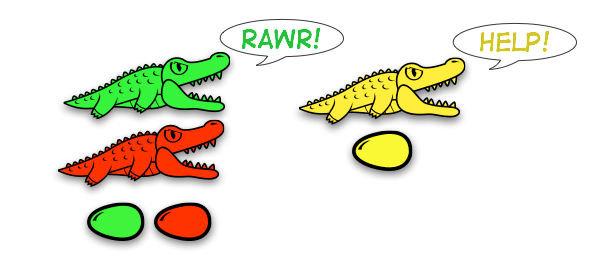
\includegraphics[width=2in]{../images/alligatorEat.png}
	\caption{A reduction visualized as an alligator eating}
	\label{fig:images_alligatorEat}
\end{figure}

In Figure \ref{fig:images_alligatorOld} we see an example of the old age rule.
In Figure \ref{fig:images_alligatorOld} (a) the old alligator guards more than
one alligator and therefore works as a parenthesis. Now the green alligator
eats the red alligator. We now see in Figure \ref{fig:images_alligatorOld} (b)
that the old alligator only has the red alligator to guard, which is the
reason for that it will now die. In normal mathematical words, this means that
the parenthesis only concludes one element and is therefore useless. Figure
\ref{fig:images_alligatorOld} (c) shows the end result with the old alligator
dead.

\begin{figure}[htbp]
	\centering
		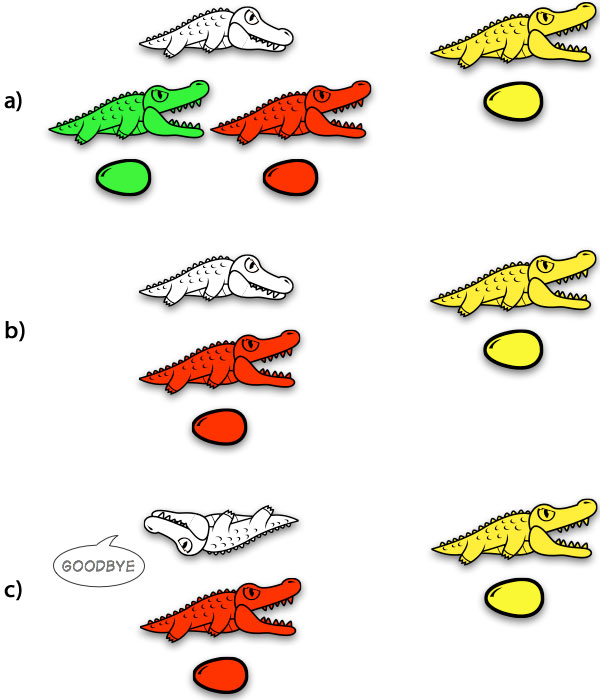
\includegraphics[width=2in]{../images/alligatorOld.jpg}
	\caption{Example of the old age rule}
	\label{fig:images_alligatorOld}
\end{figure}

``Alligator Eggs - A Puzzle Game'' does not deal with the same kind of
visualization tasks that we do in this project. It basically presents a
creative way of drawing syntax trees and a new, carnivorous terminology for
the transformations in the lambda calculus. 

The game has been implemented as a Java program, so that one does not need to
actually print out the alligators \cite{AlligatorTool}.

\section{Lambda Animator by Mike Thyer}

The ``Lambda Animator'' is a representation of lambda terms in syntax tree form. It
is implemented in Java and available online via a Java Applet
\cite{lambdaAnimatorThyer}.

\begin{figure}[!htbp]
	\centering
		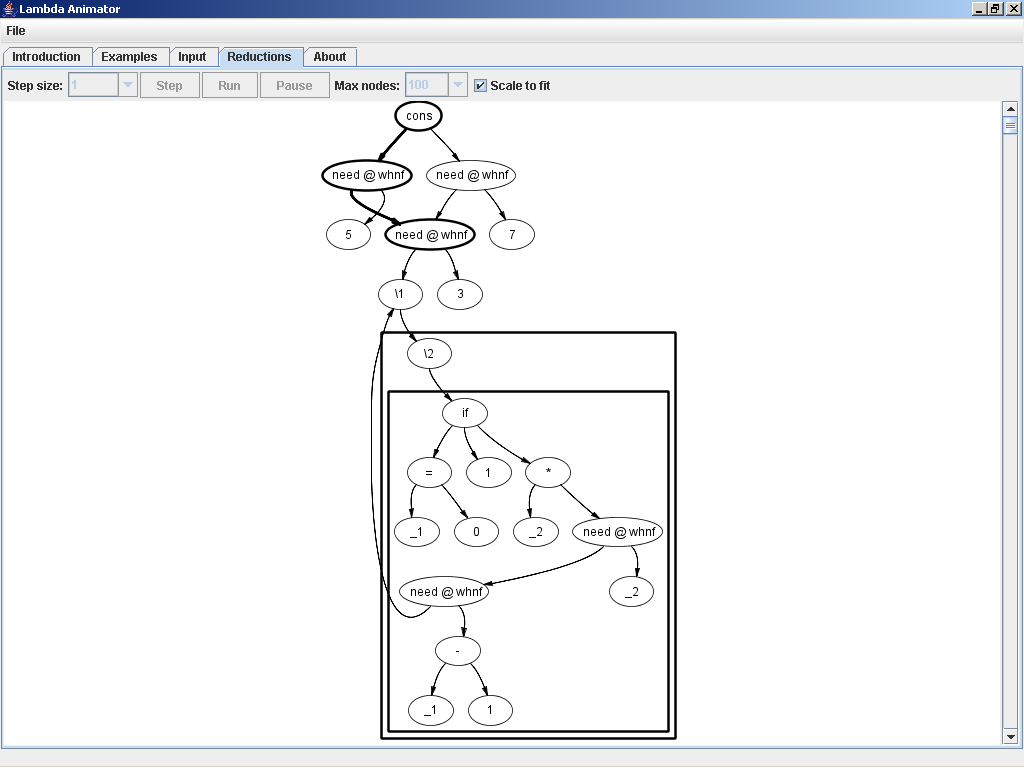
\includegraphics[scale=0.1]{../images/lambdaAnimator.png}
	\caption{Screenshot of the Lambda Animator tool}
	\label{fig:images_lambdaAnimator}
\end{figure}

The Animator does not seem very smooth and does not produce graphs that are
neither pretty nor especially visually informative, since they can be very
large. The implementation in the form of a Java applet does have some
advantages in terms of easy access to the tool, though.

It can give an reasonable overview when the lambda terms are not too complex.
In Figure \ref{fig:images_lambdaAnimatorReduction} there is an example of a
simple $\beta$-reduction. Note that the lambda calculus used in the Animator
has syntactic sugar in the form of function names etc.

\begin{figure}[!htbp]
	\centering
		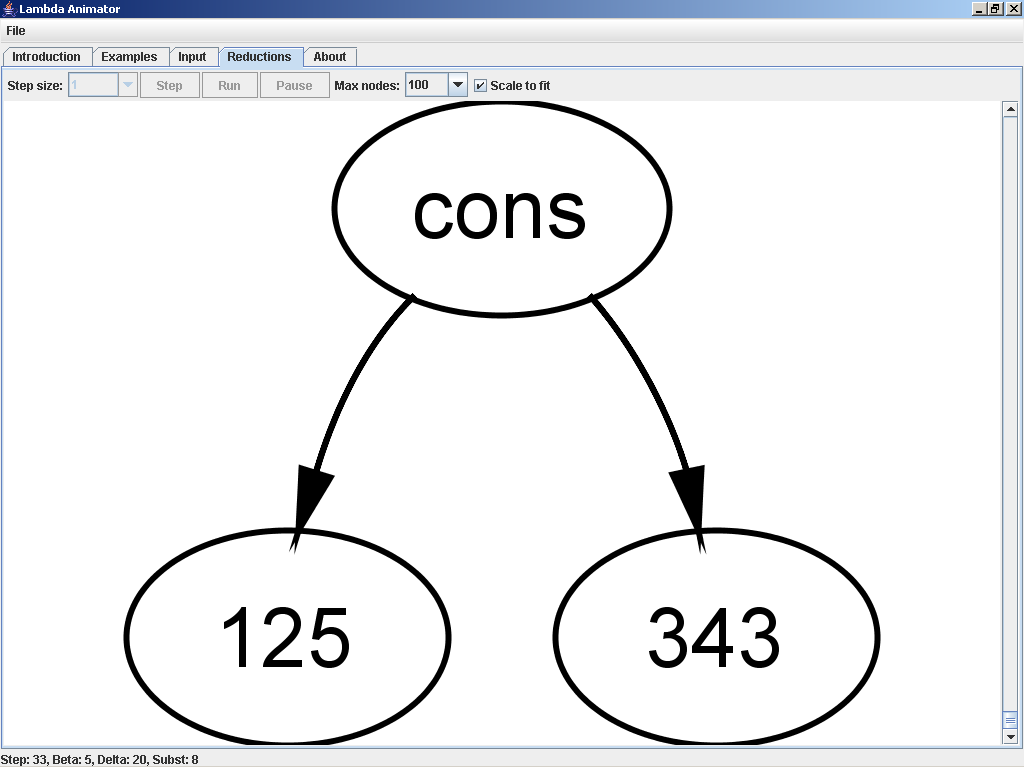
\includegraphics[scale=0.25]{../images/lambdaAnimatorReduction.png}
	\caption{Example of a simple $\beta$-reduction in the Lambda Animator}
	\label{fig:images_lambdaAnimatorReduction}
\end{figure}

\begin{figure}[!htbp]
	\centering
		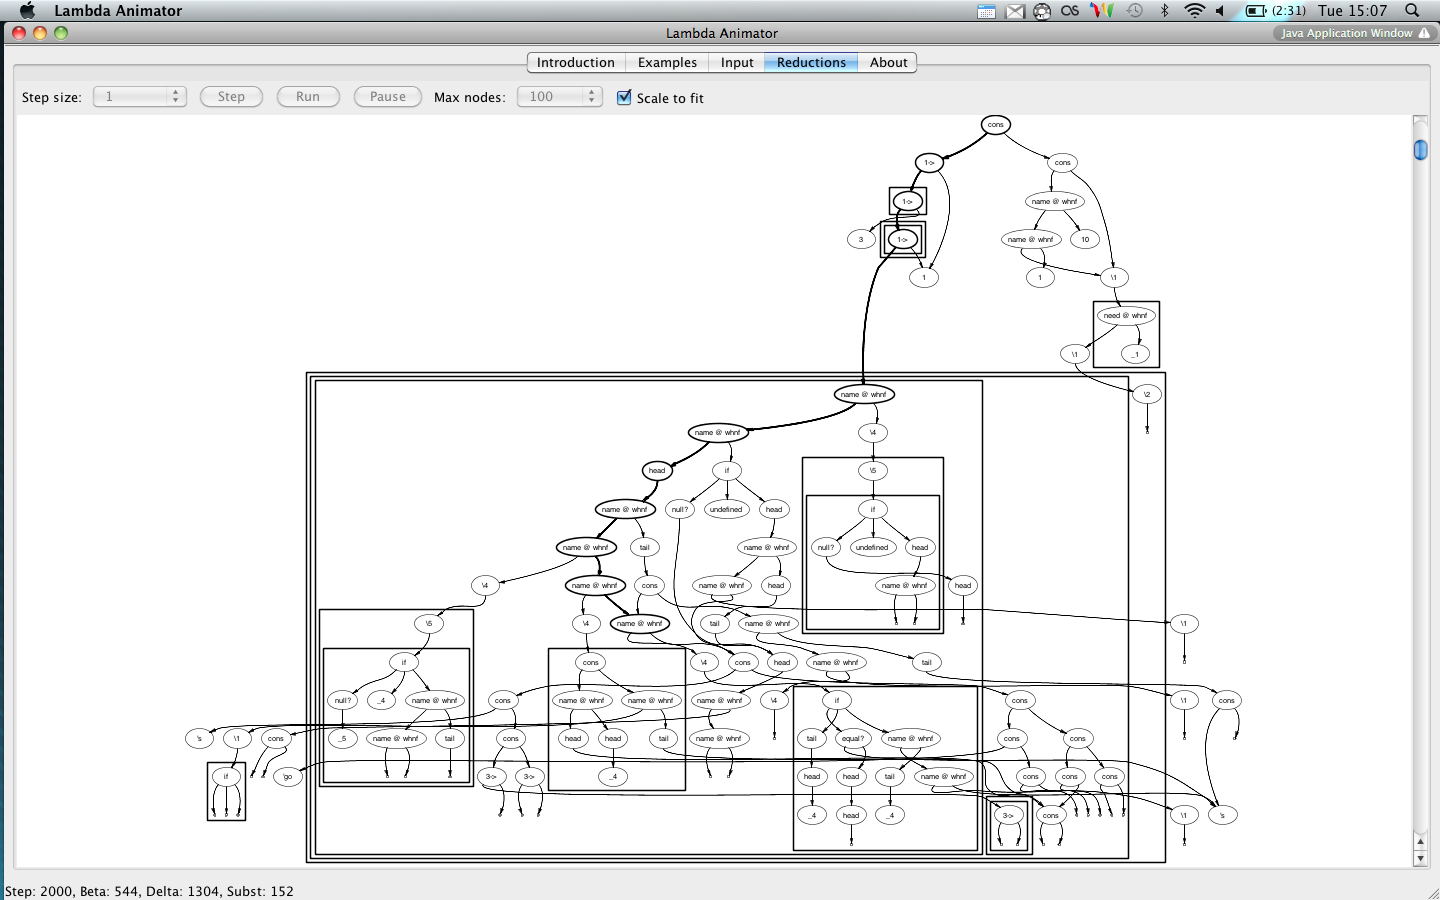
\includegraphics[scale=0.25]{../images/lambdaAnimatorComplex.png}
	\caption{Complex example in the Lambda Animator}
	\label{fig:images_lambdaAnimatorComplex}
\end{figure}

When dealing with more complex lambda terms it easily gets chaotic. In Figure
\ref{fig:images_lambdaAnimatorComplex} there is another example, in which one
can see that the informativeness seems to drastically degrade when the term
complexity is increasing.


